% ----------------------------------------------------------
\chapter{Revisão Bibliográfica}\label{cap:revisaobibliografica}
% ----------------------------------------------------------

% ----------------------------------------------------------
\section{Definições}
% ----------------------------------------------------------

No intuito de esclarecer termos e conceitos utilizados neste trabalho, dedica-se esta seção.

% ----------------------------------------------------------
\subsection{Resíduos Sólidos Industriais}
% ----------------------------------------------------------

De acordo com o \gls{PNRS}, resíduos sólidos são todo:

\begin{citacao}
	"Material, substância, objeto ou bem descartado resultante de atividades humanas em sociedade, cuja destinação final se procede, se propõe proceder ou se está obrigado a proceder, nos estados sólido ou semissólido, bem como gases contidos em recipientes e líquidos cujas particularidades tornem inviável o seu lançamento na rede pública de esgotos ou em corpos d’água, ou exijam para isto soluções técnicas ou economicamente inviáveis em face da melhor tecnologia disponível. \cite[Art. 3º, ítem XVI]{brasil_lei_nodate}"		
\end{citacao}

No contexto deste trabalho, considera-se em especial \gls{RSI}s, conforme mencionado no website do \gls{SINIR} como: resíduos gerados nos processos produtivos e instalações industriais \cite{sinir_sinir_nodate}.

% ----------------------------------------------------------
\subsection{Direcionamento de resíduos sólidos industriais}
% ----------------------------------------------------------

Em consonância com a seção V do \gls{PNRS} que responsabiliza os geradores de resíduos enquandrados nas alíneas  “e”, “f”, “g” e “k” do inciso I do art. 13 — sendo “f” relativa aos geradores de \gls{RSI}s — a elaborarem o \gls{PGRS}, o qual aponta e descreve as ações realizadas para minimizar a geração de resíduos na fonte e procedimentos relacionados à movimentação dos resíduos até que cheguem à destinação ambientalmente adequada.

A \autoref{fig:Fig_1} ilustra as principais destinações finais de resíduos em \gls{SC} por município. É possível observar a ausência de lixões em todo estado, bem como a vasta quantidade de aterros sanitários, ambos indicativos de uma boa condução no que tange a descarte de resíduos.

Apesar de não termos lixões no estado, entende-se que devem ser traçadas alternativas que reincorporem parte desses resíduos na cadeia produtiva. Nas próximas seções, descrevem-se, além das mencionadas na \autoref{fig:Fig_1}, outras tecnologias de destinação dos resíduos sólidos para conhecimento.


\begin{figure}[h]
	\caption{\label{fig:Fig_1} Tratamento e Disposição Final de Resíduos em \gls{SC}.}
	\begin{center}
		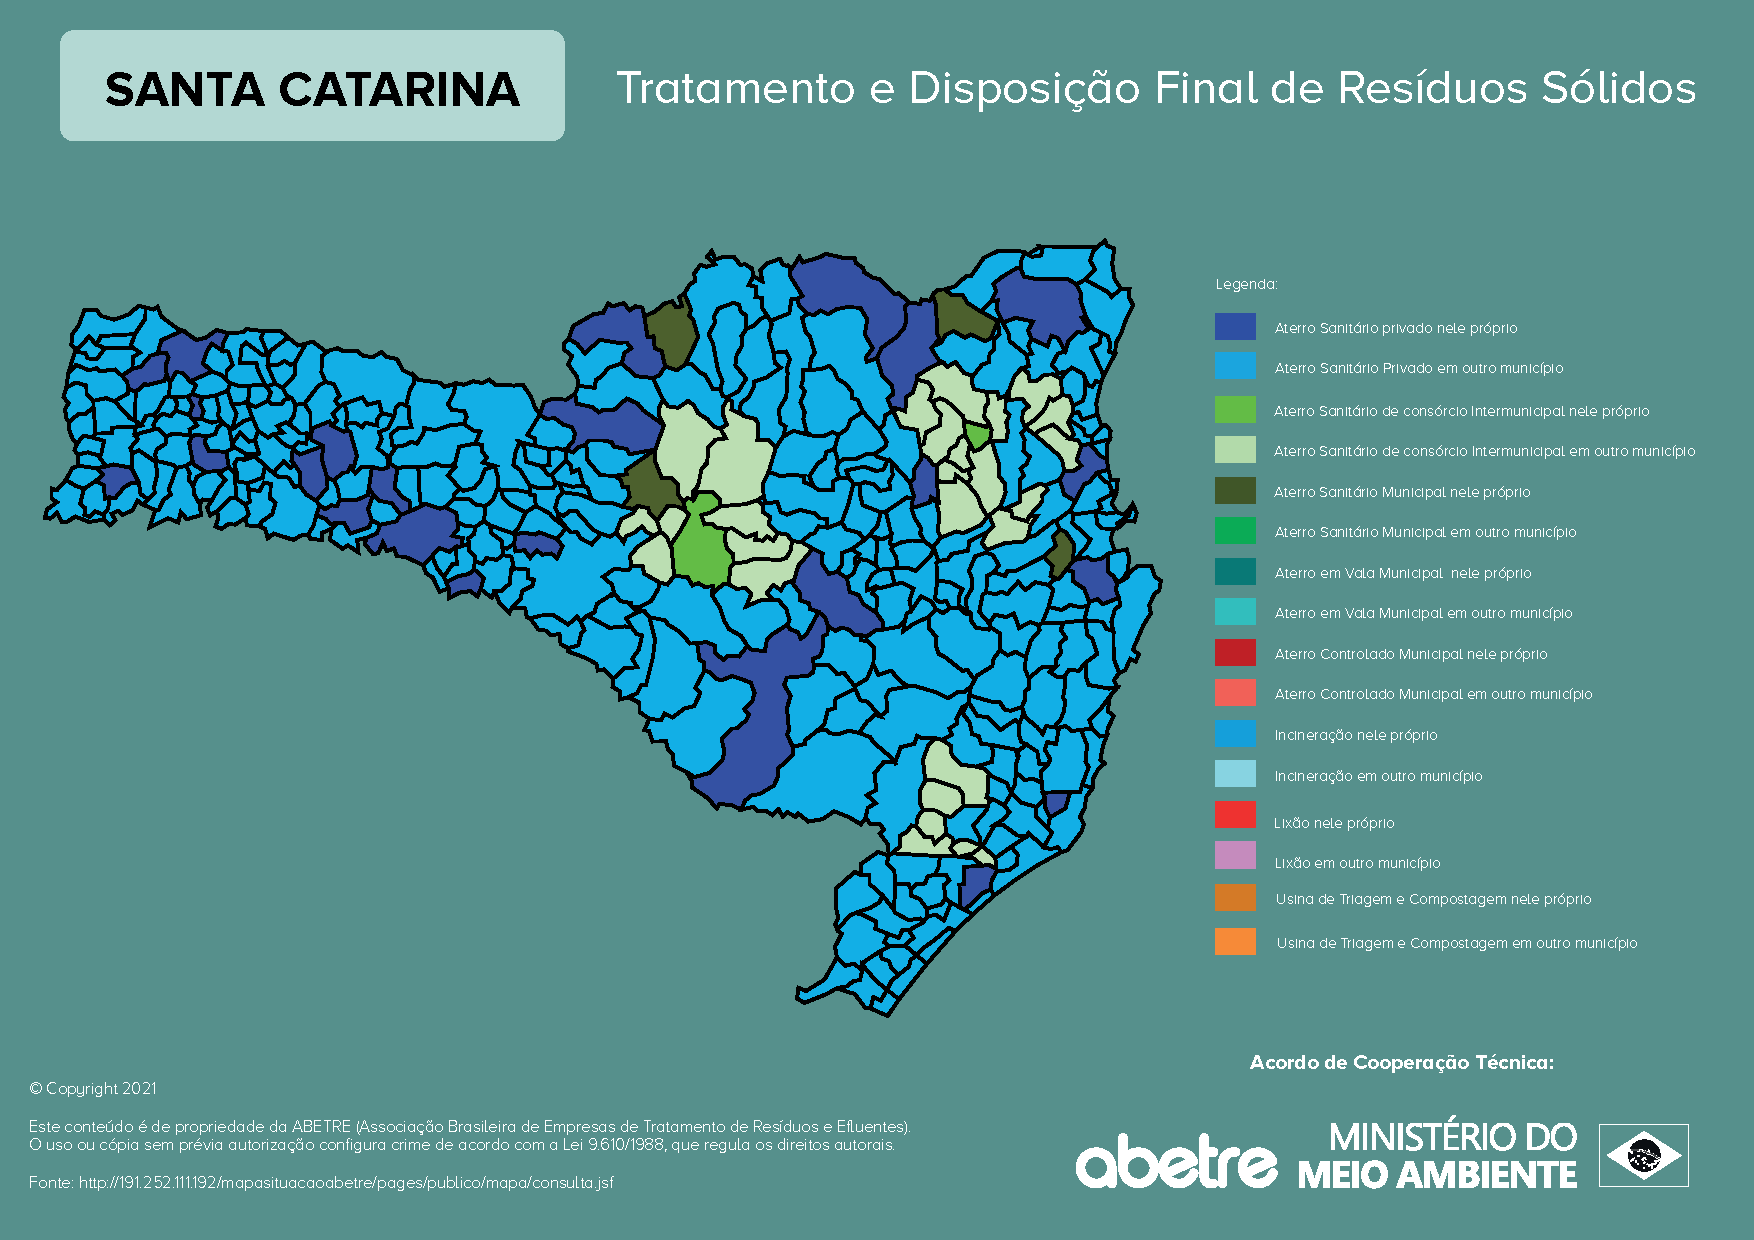
\includegraphics[scale=0.52]{images/abetre_sc.pdf}
	\end{center}
	\fonte{\gls{ABETRE}}
\end{figure}

\pagebreak
% ----------------------------------------------------------
\subsubsection{Aterro}
% ----------------------------------------------------------

Uma das destinações mais comuns no país, são áreas de armazenamento de resíduos \cite{diagnostico_cristine}:
\begin{itemize} 
	\item \textbf{Lixão:} a céu aberto;
	\item \textbf{Aterros Controlados:} em locais sem impermeabilização do solo;
	\item \textbf{Aterros Sanitários:} em espaço com engenharia dedicada à maior compactação dos resíduos e menor dano possível ao meio ambiente;
\end{itemize}
% ----------------------------------------------------------
\subsubsection{Tratamentos térmicos}
% ----------------------------------------------------------
Bastante utilizados no ramo da saúde \cite{diagnostico_cristine}:
\begin{itemize} 
	\item \textbf{Autoclave:} consiste na desinfecção dos resíduos através do aquecimento a uma temperatura elevada em contato com o vapor de água superaquecido;
	\item \textbf{Incineração:} queima dos resíduos a temperaturas superiores a 1000 °C numa atmosfera com oxigênio;
	\item \textbf{Microondas:} exposição dos resíduos à radiação eletromagnética de alta frequência;
	\item \textbf{Pirólise:} realiza-se o aquecimento dos materiais acima de 1000 °C numa atmosfera sem oxigênio;
\end{itemize}

% ----------------------------------------------------------
\subsubsection{Blendagem e coprocessamento}
% ----------------------------------------------------------

A \textbf{blendagem} é um processo de mistura de resíduos (\textit{"blends"}) a fim de gerar um produto alternativo ou matéria prima. Geralmente são misturados resíduos específicos para substituir ou reduzir o uso de uma matéria prima, barateando o processo. 

O \textbf{coprocesamento} utiliza os \textit{"blends"} de alto poder calorífico para destruição térmica dos resíduos em fornos de cimento resultando numa economia energética e de matéria prima \cite{noauthor_destinacao_nodate}


% ----------------------------------------------------------
\subsubsection{Compostagem}
% ----------------------------------------------------------

Trata-se de um método aeróbio de reciclagem e tratamento de resíduos orgânicos que busca reproduzir as condições observadas no processo natural de degradação da matéria orgânica \cite{diagnostico_cristine}.

% ----------------------------------------------------------
\subsubsection{Descontaminação de lâmpadas}
% ----------------------------------------------------------
Está relacionado à logística reversa das lâmpadas que contém mercúrio em sua composição. Consiste normalmente em pontos de entrega em estabelecimentos comerciais do país. As lampadas coletadas são transportadas e destinadas a recicladores homologados \cite{noauthor_legislacao_2023}.

% ----------------------------------------------------------
\subsubsection{Fins Didáticos}
% ----------------------------------------------------------

Trata da disposição de resíduos para utilização em unidades organizacionais. Por se tratar de uma movimentação de bem móvel entre organizações e órgãos da União fica regido pelo DECRETO Nº 10.340, 2020 \cite{brasil_decreto_2020}

% ----------------------------------------------------------
\subsubsection{Reciclagem} 
% ----------------------------------------------------------
De acordo com a \gls{PNRS}, reciclagem é o “processo de transformação dos resíduos sólidos que não seriam aproveitados, com mudanças em seus estados físico, físico-químico ou biológico, de modo a atribuir características ao resíduo para que ele se torne novamente matéria-prima ou novos produtos [...]” \cite[Art 3º, ítem XIV]{brasil_lei_nodate}.

% ----------------------------------------------------------
\subsubsection{Recuperação Energética}
% ----------------------------------------------------------

A recuperação energética é um processo que utiliza a energia contida nos resíduos sólidos para gerar eletricidade, calor ou combustíveis alternativos através da digestão anaeróbia, recuperação de gás de aterro sanitário, incineração e coprocessamento \cite{abren_abren_2021}

% ----------------------------------------------------------
\subsubsection{Rerrefino} 
% ----------------------------------------------------------

É o processo relacionado a recolhimento, coleta e destinação final de \gls{OLUC} de modo a aproveitar ao máximo seus constituintes e não causar danos ambientais \cite{diagnostico_cristine}.

% ----------------------------------------------------------
\subsubsection{Tratamento de Efluentes}
% ----------------------------------------------------------

Diz respeito à \gls{ETE}, que são: “unidades operacionais do sistema de esgotamento sanitário que através de processos físicos, químicos ou biológicos removem as cargas poluentes do esgoto, devolvendo ao ambiente o produto final,  efluente tratado, em conformidade com os padrões exigidos pela legislação ambiental.” \parencite{casan_ete_2023}

\subsubsection{Uso Agrícola}

É pertinente à utilização de resíduos como fertilizantes, sejam de origem agropecuária, urbana ou industrial. O uso de resíduos como fertilizantes atende requisitos da economia circular, economia verde e resíduo zero. \cite{diagnostico_cristine}


% ----------------------------------------------------------
\section{Classificações de resíduos sólidos industriais}
% ----------------------------------------------------------

A classificação de resíduos sólidos industriais é um processo fundamental que visa identificar suas características, riscos potenciais e formas apropriadas de tratamento e destinação. 

% ----------------------------------------------------------
\subsection{ABNT NBR 10004:2004}
% ----------------------------------------------------------

Para efeitos da norma ABNT NBR 10004:2004 Resíduos Sólidos — Classificação \cite{abnt_abnt_2004}, os resíduos são classificados com base no seu risco ao meio ambiente e à saúde. Os códigos possuem uma letra e três números. A classicação pode ser encontrada no \autoref{qua:Quadro_1}

\begin{quadro}[htb]
	\centering
	\caption{\label{qua:Quadro_1} Classificação de Resíduos Sólidos de acordo com a ABNT NBR 10004.}	
	\resizebox{\textwidth}{!}{\begin{tabular}{|l|p{11cm}|}
		\hline
		\textbf{Resíduos classe I — Perigosos} & São aqueles que em detrimento das características físicas, químicas e biológicas apresentam riscos a saúde e meio ambiente.  \\ \hline
		\textbf{Resíduos classe II — Não perigosos}        & São resíduos que não apresentam periculosidade aparente, exemplos são: sucatas, madeira, papel e papelão, borracha, areia de fundição, bagaço de cana.\\ \hline
		\textbf{Resíduos classe II A — Não inertes}          & São os resíduos que não se encaixam na classe II B. \\ \hline
		\textbf{Resíduos classe II B — Inertes}        & Quaisquer resíduos que, segundo normas auxiliares (ABNT NBR 10007 e ABNT NBR 10006) não tiverem nenhum de seus constituintes solubilizados e concentrações superiores aos padrões de potabilidade de água, excetuando-se aspecto, cor, turbidez, dureza e sabor. \\ \hline
	\end{tabular}}
	\fonte{\textcite{abnt_abnt_2004}.}
\end{quadro}


% ----------------------------------------------------------
\subsection{CONAMA}
% ----------------------------------------------------------

A RESOLUÇÃO CONAMA nº 358, 2005 \cite{noauthor_legislacao_conama_2005} com vistas a preservar a saúde pública e a qualidade do meio ambiente, dispõe sobre o tratamento e a disposição final dos resíduos dos serviços de saúde e dá outras providências, como a classificação dos resíduos em cinco grupos (A, B, C, D e E), conforme \autoref{qua:Quadro_2}

\begin{quadro}[htb]
	\centering
	\caption{\label{qua:Quadro_2} Classificação de Resíduos Sólidos de acordo com a CONAMA.}	
	\resizebox{\textwidth}{!}{\begin{tabular}{|l|p{11cm}|}
		\hline
		\textbf{I — Grupo A} & Resíduos com a possível presença de agentes biológicos que, por suas características de maior virulência ou concentração, podem apresentar risco de infecção.  \\ \hline
		\textbf{II — Grupo B}        & Resíduos contendo substâncias químicas que podem apresentar risco à saúde pública ou ao meio ambiente, dependendo de suas características de infl amabilidade, corrosividade, reatividade e toxicidade\\ \hline
		\textbf{III — Grupo C}          &  Quaisquer materiais resultantes de atividades humanas que contenham radionuclídeos em quantidades superiores aos limites de eliminação especifi cados nas normas da Comissão Nacional de Energia Nuclear-CNEN e para os quais a reutilização é imprópria ou não prevista. \\ \hline
		\textbf{IV — Grupo D}        & Resíduos que não apresentem risco biológico, químico ou radiológico à saúde ou ao meio ambiente, podendo ser equiparados aos resíduos domiciliares. \\ \hline
		\textbf{V — Grupo E}        & Materiais perfurocortantes ou escarifi cantes, tais como: lâminas de barbear, agulhas, escalpes, ampolas de vidro, brocas, limas endodônticas, pontas diamantadas, lâminas de bisturi, lancetas; tubos capilares micropipetas; lâminas e lamínulas; espátulas; e todos os utensílios de vidro quebrados no laboratório (pipetas, tubos de coleta sanguínea e placas de Petri) e outros similares. \\ \hline
	\end{tabular}}
	\fonte{\textcite{noauthor_legislacao_conama_2005}.}
\end{quadro}

% ----------------------------------------------------------
\subsection{IBAMA}
% ----------------------------------------------------------

O \gls{IBAMA} por meio da INSTRUÇÃO NORMATIVA Nº 13, 2012 \cite{noauthor_instrucao_ibama} define que “A classificação de resíduos sólidos envolve a identificação do processo ou atividade que lhes deu origem, de seus constituintes e características, e a comparação destes constituintes com listagens de resíduos e substâncias cujo impacto à saúde e ao meio ambiente é conhecido.”.

Trata-se da classificação mais completa no Brasil até o momento de publicação desse trabalho, é também a referência para o \gls{MTR}. A estrutura segue um padrão de capítulo, subcapítulo, indicador de periculosidade e resíduo, consolidando no fim o código do resído, conforme \autoref{fig:Fig_2}. Atualmente, existe um total de 878 códigos classificando os resíduos sólidos; existe uma lista disponível no \href{https://www.gov.br/ibama/pt-br/assuntos/emissoes-e-residuos/residuos/arquivos?b_start:int=0}{site do IBAMA} em \href{https://www.gov.br/ibama/pt-br/assuntos/emissoes-e-residuos/residuos/arquivos/ibama-lista-brasileira-de-residuos-solidos.xls/view}{.xls} e \href{https://www.gov.br/ibama/pt-br/assuntos/emissoes-e-residuos/residuos/arquivos/ibama-lista-brasileira-de-residuos-solidos.doc/view}{.doc}

\begin{figure}[h]
	\caption{\label{fig:Fig_2} Exemplo de construção código de identificação de resíduo do IBAMA.}
	\begin{center}
		\includegraphics[scale=0.8]{images/exemplo-codigo-ibama.png}
	\end{center}
	\fonte{\gls{IBAMA}}
\end{figure}


% ----------------------------------------------------------
\section{Principais atividades econômicas de SC}
% ----------------------------------------------------------

% ----------------------------------------------------------
\section{Coleta de dados sobre resíduos sólidos industriais no Brasil}
% ----------------------------------------------------------

% ----------------------------------------------------------
\subsection{Manifesto de Transporte de Resíduos}
% ----------------------------------------------------------

% ----------------------------------------------------------
\subsection{CTF/RAPP}
% ----------------------------------------------------------

% ----------------------------------------------------------
\subsection{Programa Lixão Zero}
% ----------------------------------------------------------

% ----------------------------------------------------------
\subsection{SINIR}
% ----------------------------------------------------------

% ----------------------------------------------------------
\section{Estado da arte}
% ----------------------------------------------------------
